\section{Evaluation}
\label{sec:results}

We evaluate over \Nruns{} agentic runs---\Ntasks{} \textsc{ParEval} OpenMP tasks
spanning \Ntypes{} problem families, \Nmodels{} models, and three tool levels---and
report configuration-robust correctness (Eq.~\ref{eq:R}) with Wilson 95\%
confidence intervals throughout. The evaluation is built around a single question:
does a verifier that \emph{observes} many thread counts make an agent's parallel
code more robust than one that observes a single configuration? Our answer is a
precise, instrumented \emph{null}---the differential verifier changed no
outcome---paired with a positive control that proves the instrument is not inert.
We report the null prominently because we designed the study to detect its
opposite, and it did not appear.

\subsection{The Measurement Is a Thread Sweep, Not a Single Run}
Figure~\ref{fig:sweep} contains the study in one plot. For every generated program
we record the validation pass-rate at each thread count $\tau\in\{1,2,4,8\}$
against the serial oracle. Robust model code (green) is \emph{flat}: a program that
is correct at one thread stays correct at eight. The red curve is the failure this
paper is about, and it is not hypothetical---it is a program an open-weights model
actually shipped (Section~\ref{sec:crosscap}): a shared-bin histogram, correct at
one thread and collapsing above it. The title of this paper is the gap between
those two curves. A single-configuration check---\textsc{ParEval}'s default and an
ordinary agent's execute-and-fix signal---samples only the leftmost point, where
the two curves coincide; the differential verifier samples the whole line. For the
frontier models the two curves stayed together, because those models did not write
programs that live in the gap; the red curve shows what happens when a model
does.

\begin{figure}[t]
\centering
\IfFileExists{../results/figures/fig_thread_sweep.pdf}
  {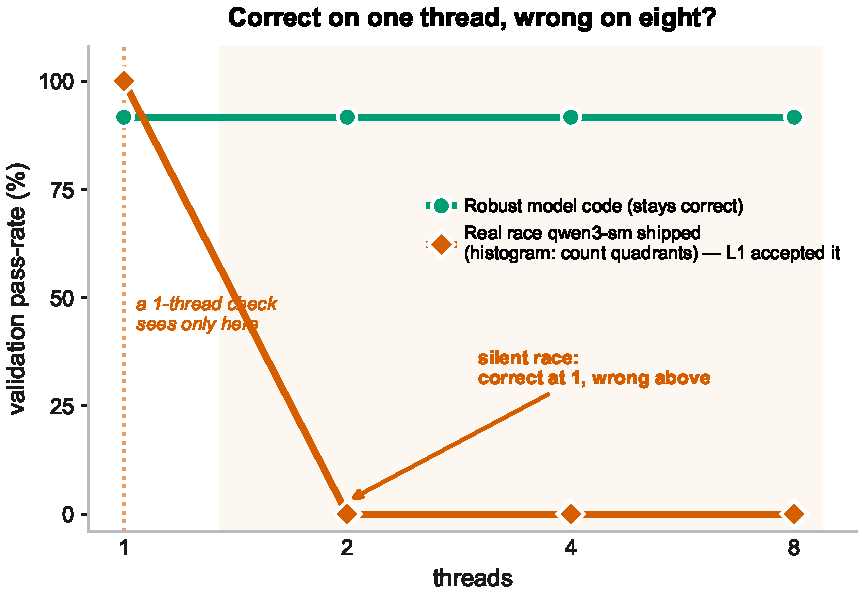
\includegraphics[width=0.92\linewidth]{../results/figures/fig_thread_sweep.pdf}}
  {\fbox{\parbox{0.8\linewidth}{\centering\vspace{2em}\textsc{[thread-sweep figure]}\vspace{2em}}}}
\caption{The study in one plot. Validation pass-rate versus thread count. Robust
model code (green) stays correct at every thread count; the red curve is a
\emph{real} silent race an open-weights model shipped---a shared-bin histogram
that is correct on one thread and wrong on two, four, and eight
(Section~\ref{sec:crosscap}), which the execute-once tool accepted. A one-thread
check sees only $\tau{=}1$ (shaded region is invisible to it).}
\label{fig:sweep}
\end{figure}

\subsection{The Parallel-Correctness Gap---Where It Was Not}
The decisive quantity for a differential verifier is how many generated programs
are of the \emph{silent-race} kind: correct at $\tau{=}1$ yet wrong at some higher
thread count. Across all \Ntasks{}$\times$\Nmodels{} task--model cells we observed
\NfailRace{} such programs. When the models were wrong they were wrong already on a
single thread---never only at higher thread counts: of \Nfail{} failing programs
under the strongest tool level, \NfailSemantic{} disagreed with the reference
already at $\tau{=}1$ and \NfailCompile{} failed to compile; \NfailRace{} were
races. As Section~\ref{sec:hetero} details, most of the $\tau{=}1$ disagreements are
a specification-ambiguity artifact on the scan family (correct parallel code, indexed
against an ambiguous prompt); the genuine residue is a single reduce task.
Where a data race was the natural pitfall---shared
histogram bins, a graph accumulator---the models pre-empted it with the correct
OpenMP idiom (a \texttt{reduction} or an \texttt{atomic}), and those tasks were
robust at every thread count. The gap we set out to measure was, for these models
on these tasks, empty.

\subsection{Tool Ablation: The Repair Loop Helps; The Verifier's Granularity Does Not}
\label{sec:ablation}
Figure~\ref{fig:ablation} and Table~\ref{tab:ablation} report the ablation
(Section~\ref{sec:agent}): the same agent at three tool levels differing only in
the observation the tool returns. Single-shot generation (L0) is robustly correct
\Lzerorate{} of the time (95\% CI \Lzeroci{}). Adding a repair loop driven by an
\emph{execute-once} tool (L1) raises this to \Lonerate{} (95\% CI \Loneci{}).
Replacing that tool with the \emph{differential verifier} (L2) yields \Ltworate{}
(95\% CI \Ltwoci{})---\emph{identical} to L1
($\Delta_{\text{L2--L1}}=\LtwoOverLone{}$). The paired view is sharper than the
aggregate: of the \Npairs{} task--model cells, the number in which execute-once and
differential verification reached a \emph{different} final verdict was \Ndiffer{},
and the number that only the differential verifier rescued was \DvOnlyRescued{}.
The multi-thread signal never changed an outcome. The improvement over single-shot
is therefore attributable to the \emph{repair loop} that L1 and L2 share, not to
the granularity of the verifier: of the \NfailSingleShot{} cells not robust at L0,
execute-once repaired \EoRescued{} and the differential verifier repaired the same
\DvRescued{}. An agent can only fix what its tool lets it
see---but here both tools saw the same failures, because those failures were
visible at one thread.

\begin{figure}[t]
\centering
\IfFileExists{../results/figures/fig_ablation.pdf}
  {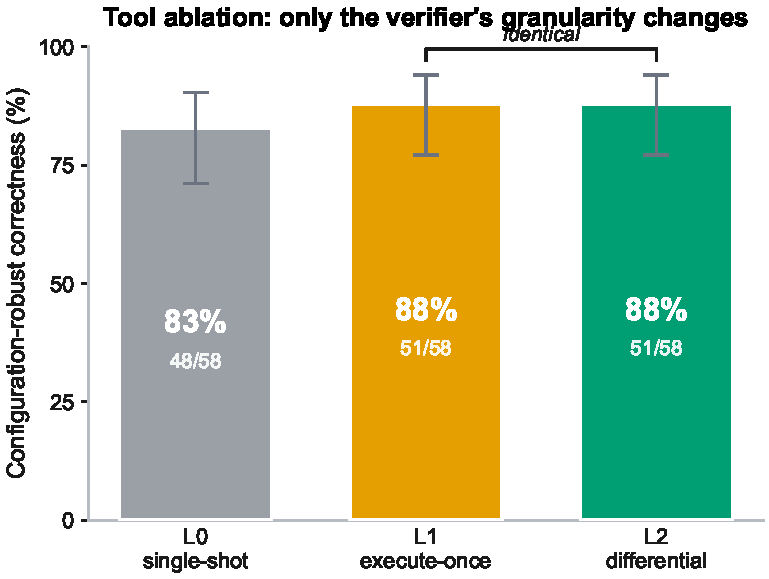
\includegraphics[width=0.82\linewidth]{../results/figures/fig_ablation.pdf}}
  {\fbox{\parbox{0.8\linewidth}{\centering\vspace{2em}\textsc{[ablation figure]}\vspace{2em}}}}
\caption{Tool ablation. Configuration-robust correctness (correct at every thread
count and repeat) with Wilson 95\% CIs; only the verification tool differs across
levels. The repair loop lifts L1 and L2 above single-shot L0, but differential
verification (L2) is indistinguishable from execute-once (L1).}
\label{fig:ablation}
\end{figure}

\begin{table}[t]
\caption{Agentic tool-ablation. Robust correctness with Wilson 95\% CIs; L1 and L2
coincide exactly.}
\label{tab:ablation}
\centering\footnotesize
\begin{tabular}{@{}lcc@{}}
\toprule
Tool level & robust correct. & 95\% CI \\
\midrule
L0 single-shot          & \Lzerorate{} & \Lzeroci{} \\
L1 execute-once         & \Lonerate{}  & \Loneci{}  \\
L2 differential verify  & \Ltworate{}  & \Ltwoci{}  \\
\bottomrule
\end{tabular}
\end{table}

\subsection{Heterogeneity Across Models and Problem Families}
\label{sec:hetero}
The equality of L1 and L2 is not an averaging artifact.
It holds for every model, including the
code-specialized one: no model produced a single case in which the thread sweep and
the single-thread check disagreed, even though the newer models failed \emph{more}
often overall---their losses were semantic and compile errors, not races.
The residual failures were concentrated and, in one family, spurious. Under
differential verification the \NfailSemantic{}+\NfailCompile{} non-race failures
break down as \NscanFail{} on the scan family and only \NgenuineFail{} elsewhere
(all one reduce task, a product-of-inverses combine). We inspected the scan
failures by hand: every model computed the reverse-indexed \emph{suffix} sum
$\text{out}[i]=\sum_{j\ge i}x_j$---a defensible reading of ``reverse prefix
sum''---which is the exact element-wise reverse of \textsc{ParEval}'s reference
(itself an inclusive scan of the reversed input). The models parallelized correctly;
they resolved an ambiguous specification against the reference's example. Excluding
this benchmark artifact, differential-verify robust correctness rises from
\Ltworate{} to \LtwoNoScan{}, and the only genuine failures are three instances of a
single reduce task---so the barrier to correct parallel code here was getting the
sequential algorithm right, not parallelizing it safely.

\subsection{Positive Control: What the Verifier Catches When the Bug Is There}
\label{sec:control}
That the differential verifier changed no outcome invites the obvious question:
does it work at all? To confirm the instrument is not inert we hand-wrote the
\emph{racy} completion a naive or weaker generator would produce for \Ninjected{}
tasks---one per hazard class: an unsynchronized shared-bin histogram, a reduction
accumulated without a \texttt{reduction} clause, and a first-match search with a
racy check-then-write on a shared index. Each is correct on one thread. We verified
each twice with the study's own tool. The execute-once check certified all
\Ninjected{} as robustly correct; the differential verifier rejected all
\NinjectedCaught{}, each failing every sweep run above one thread while passing at
one thread (Table~\ref{tab:injected}). The verifier catches exactly the failure mode a
single-thread check is blind to. The null above is therefore a statement about what
the models \emph{wrote}, not about what the verifier can \emph{see}.

\vspace{2pt}
\noindent\textbf{An independent race detector agrees.} A skeptic might still ask
whether output-differential testing at $\tau\!\le\!8$ simply lacks the power to
expose races that are present. We therefore cross-checked every one of the
\NsanTimed{} accepted programs with a happens-before detector---LLVM
Archer~\cite{archer,sword}, ThreadSanitizer instrumented with the OpenMP runtime's
OMPT annotations---which reasons about the actual synchronization, not just the
output. Archer flagged \NsanRaces{} data races in the model-written code of the
\NsanTimed{} programs the differential verifier certified robust, while correctly
reporting the race in the injected controls and in the open-model histogram of
Section~\ref{sec:crosscap} (27 stack frames in the generated code). Two independent
instruments---one output-differential, one happens-before---agree that these
accepted programs are race-free, which makes the null a statement about the code and
not an artifact of a weak detector.

\begin{table}[t]
\caption{Positive control: injected races, one per hazard class. Each is correct on
one thread; execute-once certifies all, the differential verifier rejects all.}
\label{tab:injected}
\centering\footnotesize
\begin{tabular}{@{}lcc@{}}
\toprule
Injected hazard & execute-once & differential \\
\midrule
Histogram, unsynchronized bins           & \textsc{accept} & \textsc{reject} \\
Reduction, no \texttt{reduction} clause  & \textsc{accept} & \textsc{reject} \\
First-match, racy shared index           & \textsc{accept} & \textsc{reject} \\
\bottomrule
\end{tabular}
\end{table}

\subsection{Beyond the Frontier: A Real Race the Verifier Catches}
\label{sec:crosscap}
The null above is a statement about \emph{capable} models. If differential
verification earns its place by catching silent races, the sharpest test is a
generator that actually writes them. We therefore replayed the \NraceTasks{}
most race-prone tasks through an \emph{open-weights} panel served on a
research cluster (\NopenModels{} models ranging from a 120B general model down to a
27B model), holding the harness, prompts, and differential scorer fixed, and
scored every final program over the full thread sweep
(Fig.~\ref{fig:crosscap}). The capability gradient is exactly the one the null
predicts. The larger open models behaved like the frontier: no silent races,
$L1\!=\!L2$. The smallest model did \emph{not}. On the shared-bin quadrant
histogram it emitted the canonical hazard---a \texttt{local\_bins} accumulator
declared \emph{outside} the parallel region and incremented by every thread, so
the counts are correct on one thread and lost to a data race above it. The
execute-once tool ran it once, saw a plausible histogram, and \textbf{certified
it robust}; the differential verifier ran the sweep, saw it pass at one thread
and fail at two, four, and eight, returned that diagnostic, and the agent
repaired it to a per-thread private accumulator that is robust throughout. Same
model, same task, same repair budget: the only difference was whether the tool
looked at more than one thread count. This is the first \emph{model-emitted}
instance---not an injected control---of the exact failure this paper is about.
Across the open panel the differential verifier caught \NopenRescued{} such
verified silent race(s) that the single-thread check certified, versus
\NfrontierRaces{} on the frontier panel (Fig.~\ref{fig:crosscap}b); we attribute
only genuine pass$@1$/fail$@N$ cases to the verifier and treat the remaining small
$L1$--$L2$ differences on this six-task subset as repair-sampling noise, not race
catches. The mechanism is what matters: the tool's value reappears precisely as
model capability falls.

\begin{figure*}[t]
\centering
\IfFileExists{../results/figures/fig_cross_capability.pdf}
  {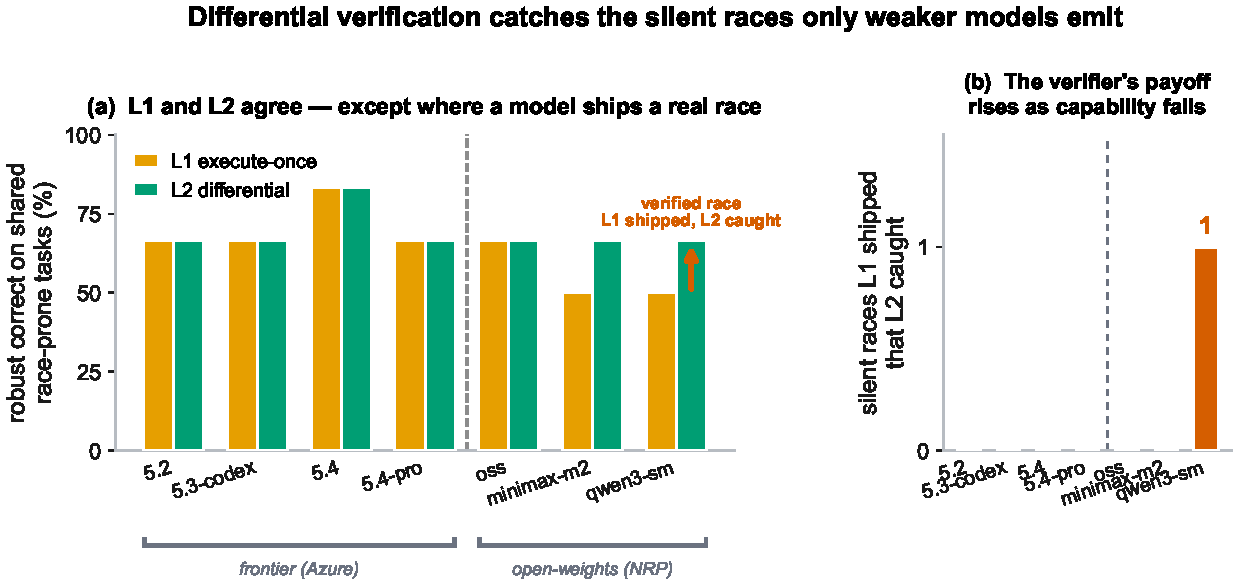
\includegraphics[width=0.94\linewidth]{../results/figures/fig_cross_capability.pdf}}
  {\fbox{\parbox{0.8\linewidth}{\centering\vspace{2em}\textsc{[cross-capability figure]}\vspace{2em}}}}
\caption{The verifier's value is capability-dependent. (a)~Robust correctness on
the shared race-prone tasks, execute-once (L1) vs.\ differential (L2), per model.
Frontier and larger open models show no meaningful gap; the arrow marks the one
\emph{verified} silent race---a shared-bin histogram the smallest open model
shipped, which L1 certified and L2 caught and repaired. (b)~Verified silent races
the single-thread check accepted that the differential verifier rejected: zero for
capable models, rising as capability falls. (Small residual L1--L2 differences in
(a) with no bar in (b), e.g.\ minimax-m2, are repair-sampling noise on this
six-task subset, not race catches.)}
\label{fig:crosscap}
\end{figure*}

\begin{table}[t]
\caption{Open-weights panel on the \NraceTasks{} race-prone tasks. Robust
correctness under L1 (execute-once) and L2 (differential); silent races each model
shipped (correct at one thread, wrong above) that L1 certified; and how many L2
caught. Only the smallest model emits a genuine race---and L2 catches it.}
\label{tab:open}
\centering\footnotesize
\begin{tabular}{@{}lcccc@{}}
\toprule
Open model & L1 & L2 & races shipped & caught by L2 \\
\midrule
gpt-oss-120B & 67\% & 67\% & 0 & 0 \\
MiniMax-M2 & 50\% & 67\% & 0 & 0 \\
Qwen3-27B & 50\% & 67\% & 1 & 1 \\
\bottomrule
\end{tabular}
\end{table}

\begin{figure}[t]
\lstset{basicstyle=\ttfamily\scriptsize,backgroundcolor=\color{codebg},
        breaklines=true,columns=fullflexible,frame=none,aboveskip=2pt,belowskip=1pt,
        escapeinside={(*@}{@*)}}
\textbf{\footnotesize L1 execute-once \textemdash{} shipped; the 1-thread check passed}
\begin{lstlisting}
void countQuadrants(vector<Point> const& pts,
                    array<size_t,4>& bins){
  bins = {0,0,0,0};
  array<size_t,4> local_bins;        // (*@\textcolor{red}{\bfseries shared: declared OUTSIDE omp parallel}@*)
  #pragma omp parallel
  { local_bins = {0,0,0,0};
    #pragma omp for nowait
    for (size_t i=0;i<pts.size();++i) local_bins[q(pts[i])]++; // (*@\textcolor{red}{race}@*)
    #pragma omp critical
    for(int k=0;k<4;k++) bins[k]+=local_bins[k]; }}
\end{lstlisting}
\vspace{-1pt}
{\scriptsize\ttfamily verifier: t1=2/2\; \textcolor{red}{t2=0/2\; t4=0/2\; t8=0/2}\;\(\Rightarrow\)\;\textcolor{red}{NOT\_ROBUST}}

\vspace{4pt}
\textbf{\footnotesize L2 differential \textemdash{} the sweep failed; the agent repaired it}
\begin{lstlisting}
  #pragma omp parallel
  { array<size_t,4> local_bins={0,0,0,0}; // (*@\textcolor{OliveGreen}{\bfseries private: declared INSIDE omp parallel}@*)
    #pragma omp for nowait
    for (size_t i=0;i<pts.size();++i) local_bins[q(pts[i])]++;
    #pragma omp critical
    for(int k=0;k<4;k++) bins[k]+=local_bins[k]; }
\end{lstlisting}
\vspace{-1pt}
{\scriptsize\ttfamily verifier: \textcolor{OliveGreen}{t1=2/2\; t2=2/2\; t4=2/2\; t8=2/2}\;\(\Rightarrow\)\;\textcolor{OliveGreen}{ROBUST}}
\caption{The verified race, from the logs (Qwen3-27B on \texttt{count\_quadrants};
transcripts released). \textbf{Top:} the execute-once agent declares the
accumulator \emph{outside} \texttt{omp parallel}---so all threads share it---but
its one-thread check passes, and it ships. \textbf{Bottom:} given the differential
tool, the same agent sees the thread sweep fail above one thread and moves the
declaration \emph{inside} the region (per-thread private), which is robust. Sweep
lines are the tool's real logged output.}
\label{fig:casestudy}
\end{figure}

\subsection{Correct but Not Parallel: The Second Axis Is Where Accepted Code Fails}
\label{sec:scaling}
The differential verifier settles the correctness axis; it is silent on the second
axis of Section~\ref{sec:secondaxis}. We measured it directly: for every one of the
\Ntimed{} programs the verifier accepted as robust, we compiled the model's code
against \textsc{ParEval}'s timing driver at a size large enough to amortize thread
overhead and recorded self-speedup $\mathcal{P}_p$ across the same sweep
$p\in\{1,2,4,8\}$ (min wall-time over repeats). The result (Fig.~\ref{fig:scaling})
is the paper's sharpest finding. Robust correctness spans \emph{the entire scaling
range}, from $7.9\times$ down to $0.33\times$---one accepted program runs three
times \emph{slower} on eight threads than on one. \PctFlatScale{} of accepted
programs ($\NflatScale{}/\Ntimed{}$) achieve under $2\times$ on eight cores; a
serial program, we reiterate, would have been accepted with identical
$\mathcal{R}{=}1$. The decisive juxtaposition (Fig.~\ref{fig:scaling}a) is two
programs the verifier certified \emph{identically} robust on the same histogram
task: one uses a per-thread \texttt{reduction} and scales $6.5\times$; the other
guards every bin update with a per-element \texttt{atomic} and, throttled by
memory-ordering contention, degrades to $0.33\times$. Correctness cannot tell them
apart; only the performance axis can.

We are deliberately careful about mechanism. The synchronization idiom a model
chose does \emph{not} cleanly predict poor scaling: programs using
\texttt{critical} mostly used it for a cheap $O(\text{threads})$ merge of
per-thread partials and scaled well (mean $\mathcal{P}_8=\MeanSpeedupCritical{}$ vs.\
$\MeanSpeedupReduction{}$ for \texttt{reduction}), so we do \emph{not} claim models
systematically over-synchronize. The defensible claim is narrower and stronger for
being exact: an output-only robustness metric is \emph{gameable by construction},
and among accepted programs measured scaling varies enormously---so correctness and
parallelism must be reported as two axes, and the second is where the failures now
live. This turns the correctness null from an endpoint into a setup: once frontier
models make race-freedom cheap, the binding constraint moves to writing code that
is not merely correct under parallelism but actually uses it.

\begin{figure*}[t]
\centering
\IfFileExists{../results/figures/fig_scaling.pdf}
  {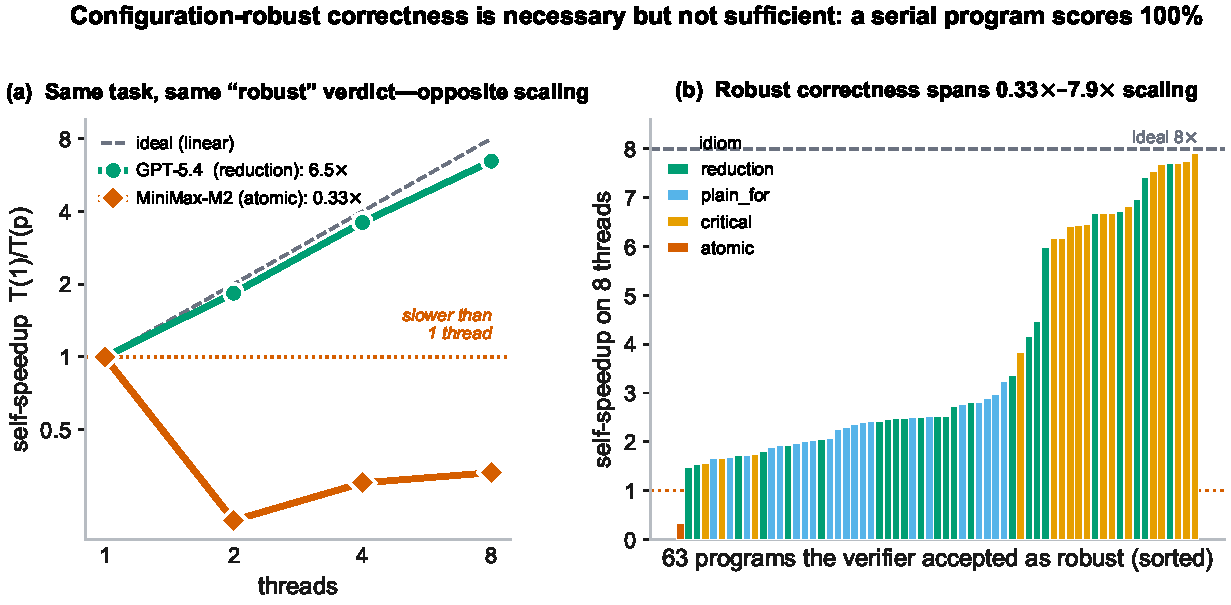
\includegraphics[width=0.96\linewidth]{../results/figures/fig_scaling.pdf}}
  {\fbox{\parbox{0.8\linewidth}{\centering\vspace{2em}\textsc{[scaling figure]}\vspace{2em}}}}
\caption{Correctness is necessary but not sufficient. (a)~Two programs the
differential verifier accepted as \emph{equally} robust on the same histogram task:
a \texttt{reduction} scales $6.5\times$; a per-element \texttt{atomic} runs
$0.33\times$---slower on eight threads than one. (b)~Self-speedup on eight threads
for all \Ntimed{} accepted programs, sorted, coloured by synchronization idiom:
robust correctness spans $0.33\times$--$7.9\times$, and a serial program would sit
at $1\times$ with the same $\mathcal{R}{=}1$. The idiom does not cleanly predict
scaling (\texttt{critical} is often a cheap merge); the point is that the
correctness axis alone cannot distinguish any of these.}
\label{fig:scaling}
\end{figure*}

\subsection{What the Null Does and Does Not Say}
The result is bounded by construction. On \Ntasks{} standard \textsc{ParEval} tasks,
\Nmodels{} strong models emit code whose correctness does not depend on the thread
count---the pass$@1$/fail$@N$ mode is absent, corroborated by an independent race
detector---so a verifier's multi-thread granularity cannot help. It does \emph{not}
say the verifier is useless: it catches the hazard the moment it is present (the
injected controls, the open-model race of Section~\ref{sec:crosscap}, and the
cliff in Fig.~\ref{fig:sweep}). Correctness verification remains the right first
gate; frontier models have simply made its cheapest form sufficient on idiomatic
tasks. The consequential gap has moved to the second axis
(Section~\ref{sec:scaling}), which no output-only test can close. We turn that gap
from a finding into a design in Section~\ref{sec:reward}: a two-axis reward, and the
selection, agentic, and post-training experiments that show what it recovers.

